\section{Expérimentation}

\subsection{Analyseur statique}

\begin{frame}{Mode de fonctionnement}

  \begin{itemize}
  \item compile vers un \texttt{.npk}
  \item enlève les types C
  \item infère des types plus sémantiques
  \end{itemize}
\end{frame}

% TODO rappel ctx
% TODO mentionner algo d'inférence
% TODO préciser au début Safespeak qu'on interdit casts etc

\begin{frame}{Traduction: C} \insertcode{tc-c.c} \end{frame}
\begin{frame}{Traduction: sans les types} \insertcode{tc-ml.c} \end{frame}
\begin{frame}{Traduction: types inférés} \insertcode{tc-ty.c} \end{frame}

    % TODO titres de ces slides à collapser en grisé

\begin{frame}{Différence entre les types C et les types inférés}
    \centering
      \begin{tabular}{ll}
          \toprule
          C/\newspeak & \langname \\ % TODO virer NPK
          \midrule
          \texttt{int} & $\tInt$ \\
          \texttt{unsigned long} & $\tInt$ \\ % TODO virer cette ligne
          \texttt{int *} (utilisé \texttt{x[i]}) & $\tInt~[~]$ \\
          \texttt{int *} (utilisé \texttt{*x}) & $\ptrK{\tInt}$ \\
          \texttt{int *} (argument syscall) & $\ptrU{\tInt}$ \\
          \bottomrule
      \end{tabular}
\end{frame}

\subsection{Utilisation sur le noyau Linux}

\begin{frame}{Analyse de 2 bugs}

    \begin{itemize}
        \item Radeon KMS
        \item \texttt{ptrace} Blackfin
    \end{itemize}
\end{frame}

% TODO déplacer cette figure dans sys de types

\begin{frame}{Code avec bug}
    % left bottom right top
    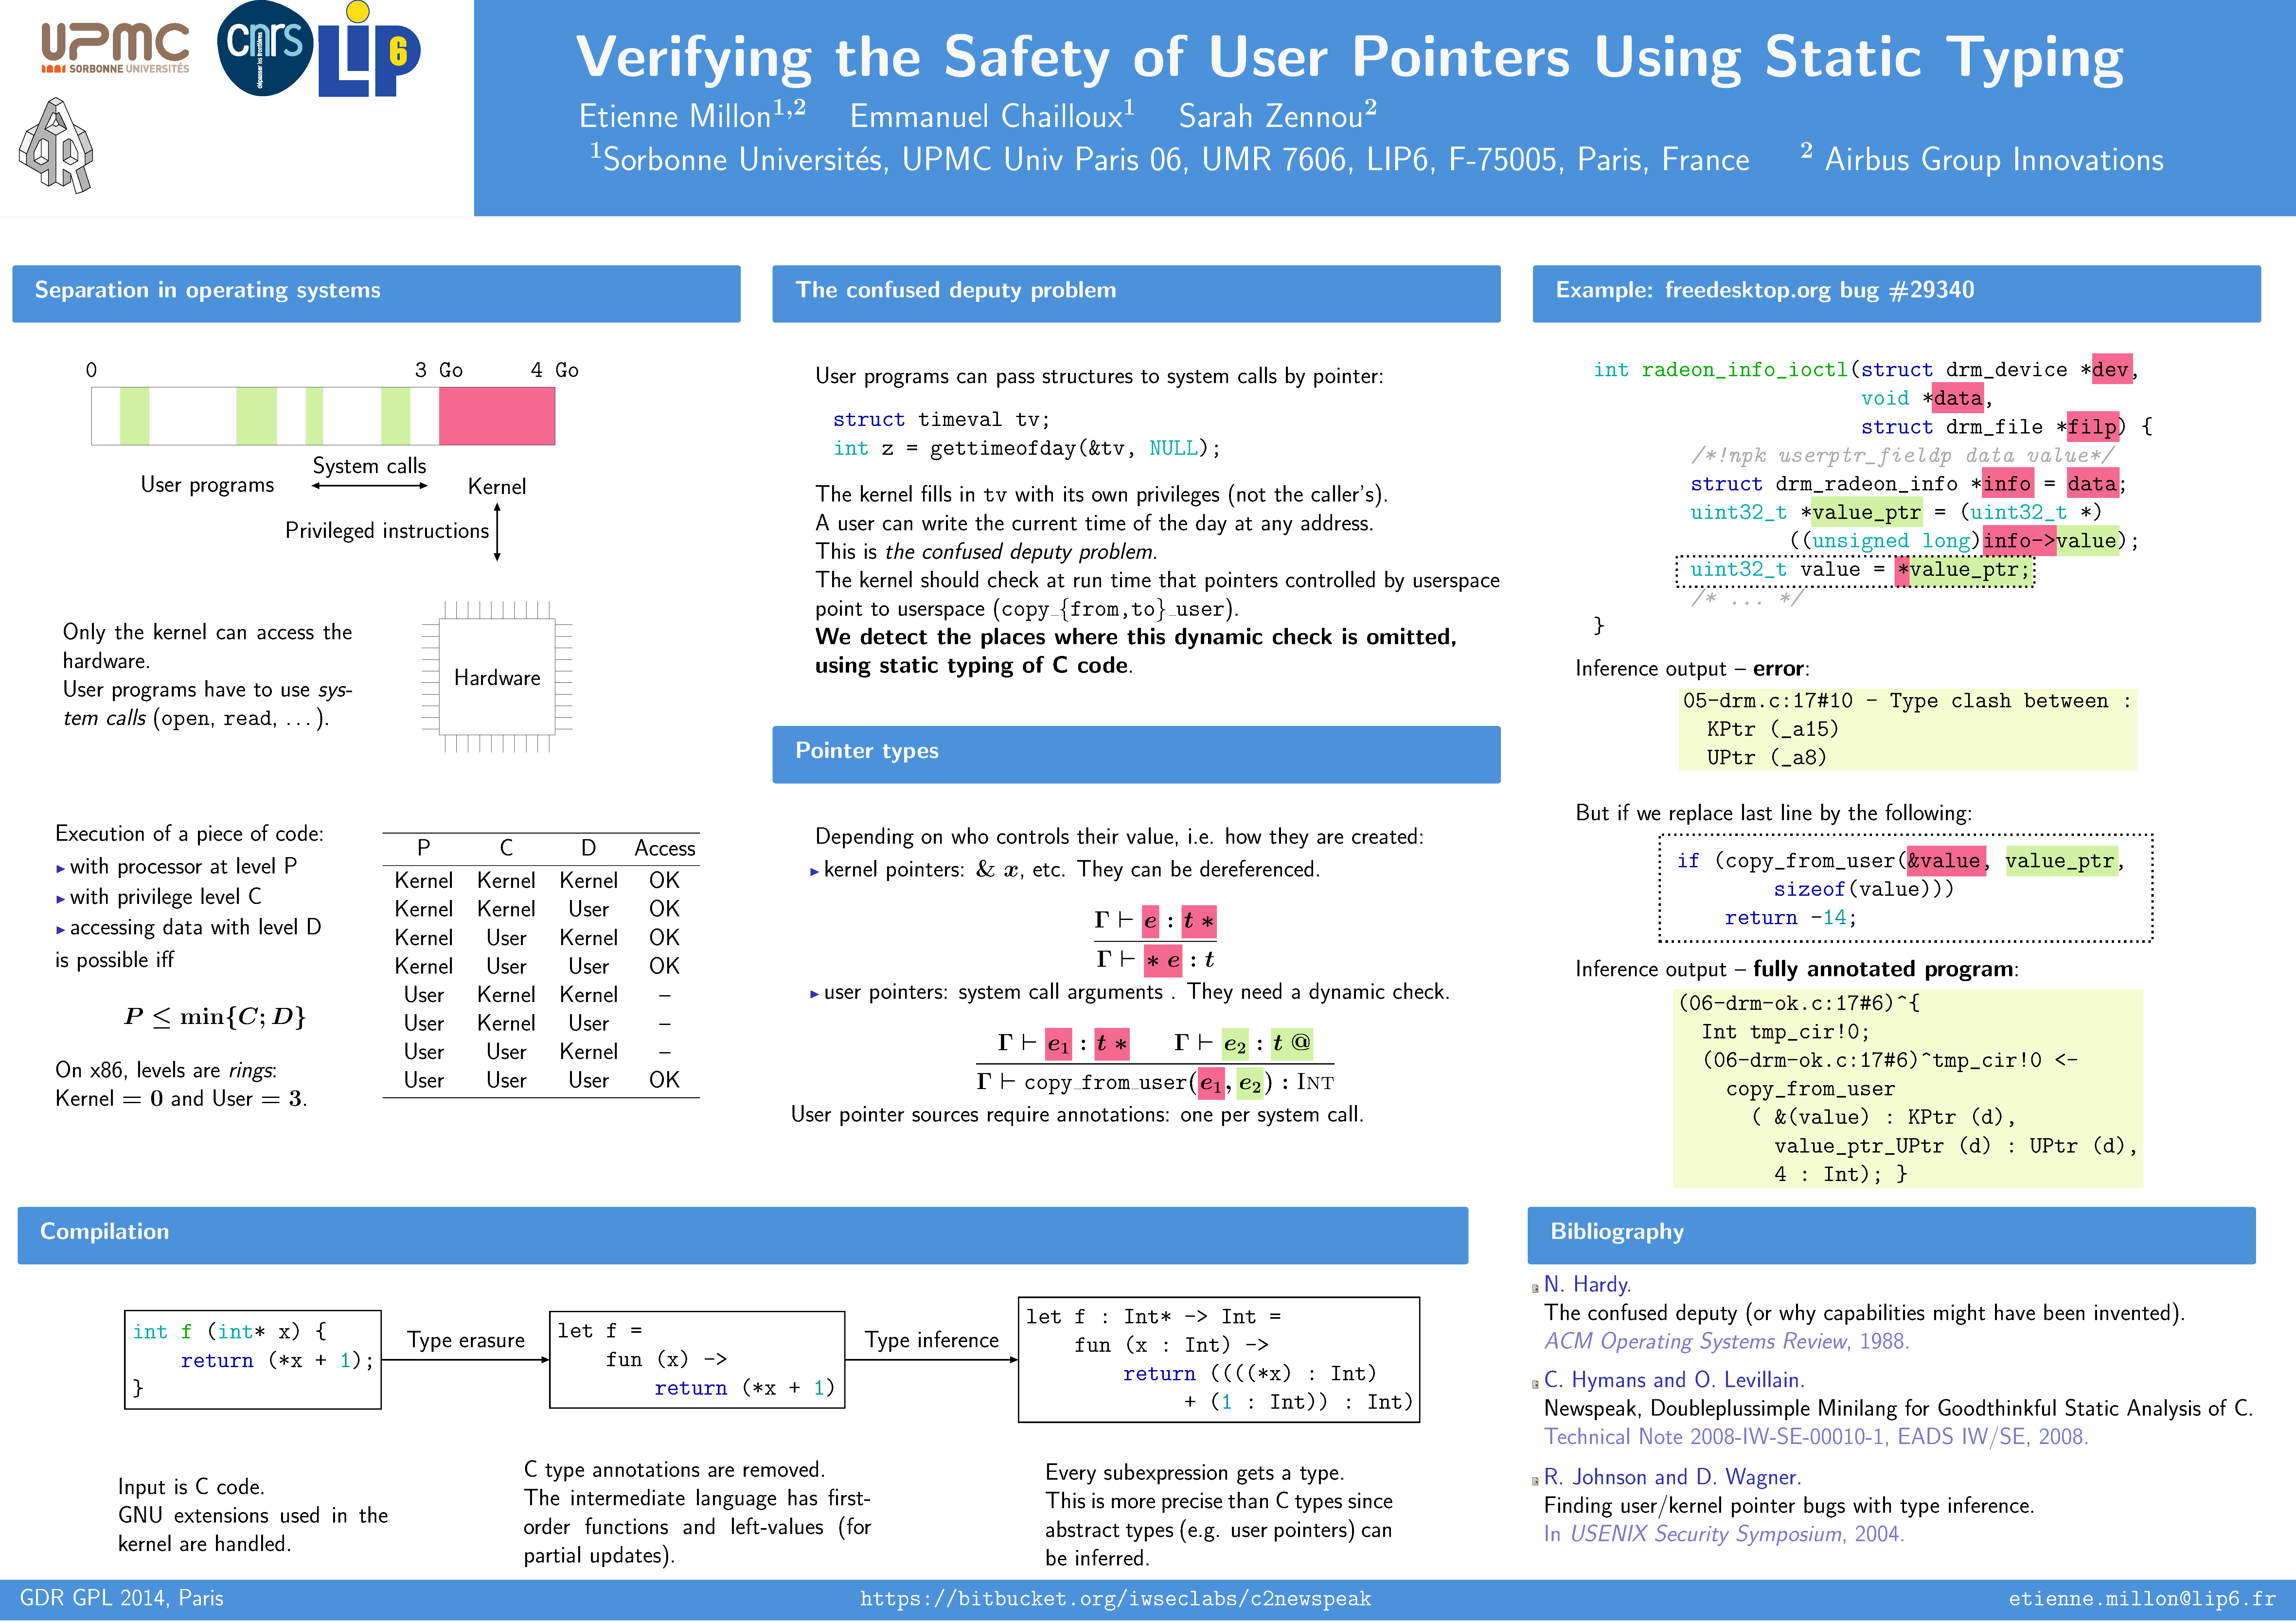
\includegraphics[trim=2300 1430 100 500,clip,width=\textwidth]{poster.pdf}
\end{frame}

\begin{frame}[fragile]{Résultat de l'algorithme d'inférence}
\begin{SaveVerbatim}{drmko}
05-drm.c:17#10 - Type clash between :
  KPtr (_a15)
  UPtr (_a8)
\end{SaveVerbatim}

\textbf{Erreur}:

\codeout{drmko} % TODO sur le même slide que précédent
% TODO ne pas parler des inconnues
\end{frame}

\begin{frame}{Code corrigé}
    % left bottom right top
    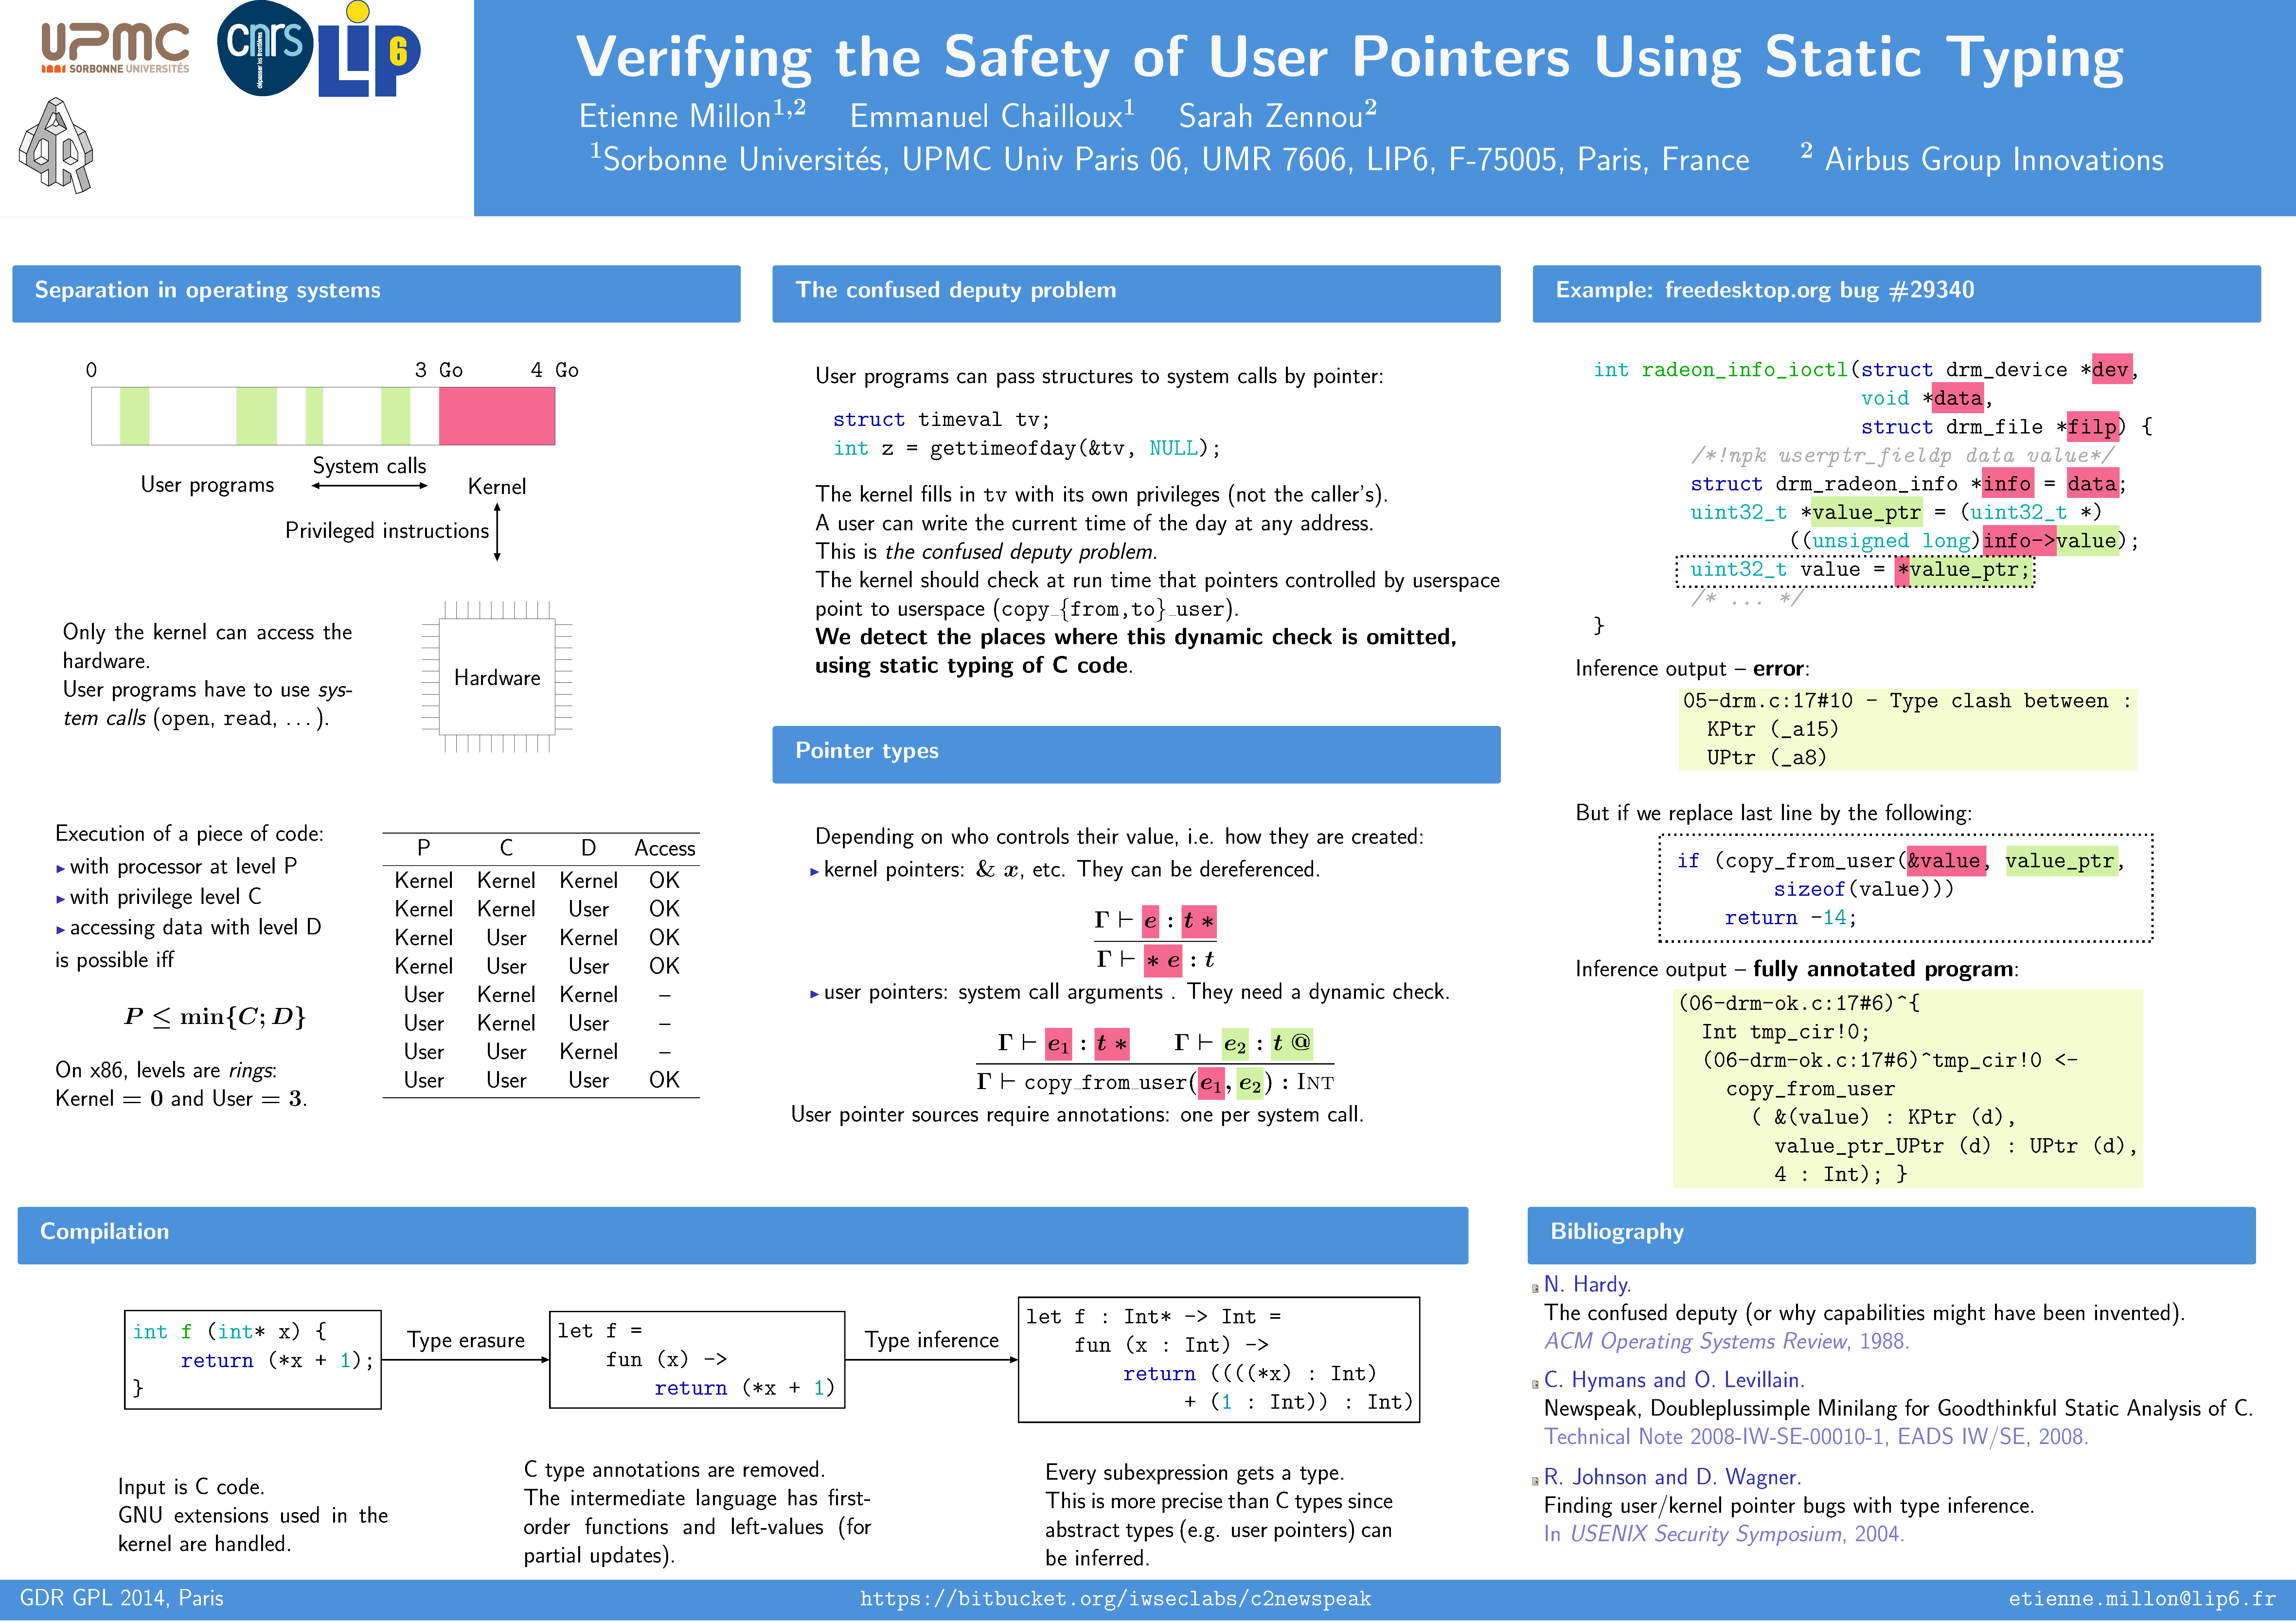
\includegraphics[trim=2300 990 100 1220,clip,width=\textwidth]{poster.pdf}
\end{frame}

\begin{frame}[fragile]{Résultat de l'algorithme d'inférence}

\textbf{Programme complètement annoté}:
% TODO annoté => étiqueté

\begin{SaveVerbatim}{drmok}
(06-drm-ok.c:17#6)^{
  Int tmp_cir!0;
  (06-drm-ok.c:17#6)^tmp_cir!0 <-
    copy_from_user
      ( &(value) : KPtr (d),
        value_ptr_UPtr (d) : UPtr (d),
        4 : Int); }
\end{SaveVerbatim}

\codeout{drmok}
\end{frame}
